\documentclass[10pt,twocolumn,twoside,slovak,a4paper]{article}
\usepackage{graphicx} % Required for inserting images


\title{Prvy textovy subor}
\author{Alžbeta Segečová}
\date{September 2024}

\begin{document}

\maketitle
Uvod do Latexu


\section{Introduction}
Toto je \textbf{prvy} uvodny text 

\section{Obsah}
Toto nebude obsah clanku pretoze musim vykonat zmenu


\section{Prve zadanie}
\textbf{Rozoberame existujuci \emph{text} , ktory... }
Kde bolo tam bolo, bol raz jeden dedko. Tento dedko mal krásnu veľkú záhradu, v ktorej pestovalvšelijakú zeleninu a chutné ovocie. Raz vyšiel dedko pred dom nadýchať sa čerstvého vzduchu. Bola jar, vtáčiky spievali, zem voňala.

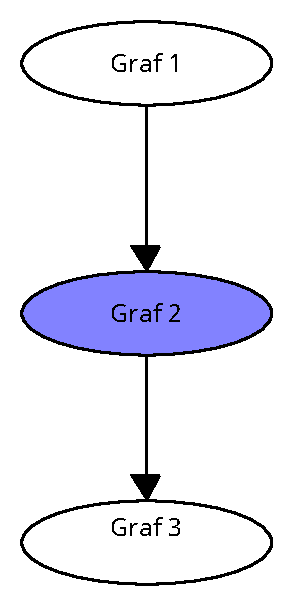
\includegraphics[width =10 cm]{diagram.pdf}


Ako je dneska krásne! – pochvaľoval si dedko. Nevdojak siahol rukou do vrecka nohavíc, a tam – semienko. Ktovie, kde sa tam vzalo!Dedko spravil pätou vo vlhkej zemi jamku a semienko do nej opatrne, ale o-pa-tr-ne vložil.
Len si rasť, maličké! Ktovie, čo z teba bude!
Semienko utešene rástlo. Najprv pustilo korienok, potom z neho vyklíčili lístky. Dedko ho polieval a okopával, ako najlepšie vedel.






\end{document}
